\documentclass[11pt,a4paper]{article}

\usepackage[a4paper,margin=2.2cm]{geometry}
\usepackage[T1]{fontenc}
\usepackage[utf8]{inputenc}
\usepackage{lmodern}
\usepackage{microtype}
\usepackage{amsmath,amssymb}
\usepackage{graphicx}
\usepackage{booktabs}
\usepackage{tabularx}
\usepackage{array}
\usepackage{float}
\usepackage{caption}
\usepackage{subcaption}
\usepackage{enumitem}
\usepackage{xcolor}
\usepackage{fancyhdr}
\usepackage{titlesec}
\usepackage[colorlinks=true,linkcolor=black,citecolor=black,urlcolor=blue!50!black]{hyperref}

\graphicspath{{../docs/images/}}

\definecolor{accent}{RGB}{140,45,30}
\titleformat{\section}{\large\bfseries\color{accent}}{\thesection}{0.6em}{}
\titleformat{\subsection}{\normalsize\bfseries}{\thesubsection}{0.6em}{}
\titlespacing*{\section}{0pt}{1.1ex plus .3ex}{0.6ex}
\titlespacing*{\subsection}{0pt}{0.9ex plus .2ex}{0.4ex}
\setlist{nosep,leftmargin=1.4em}
\captionsetup{font=small,labelfont=bf,skip=4pt}
\setlength{\parskip}{0.35em}
\setlength{\parindent}{0pt}
\setlength{\textfloatsep}{8pt plus 2pt}
\setlength{\intextsep}{8pt plus 2pt}
\renewcommand{\arraystretch}{1.12}

\pagestyle{fancy}
\fancyhf{}
\fancyhead[L]{\small CSE-4102: Computer Graphics and Image Processing Laboratory}
\fancyhead[R]{\small Roll 2107099}
\fancyfoot[C]{\small\thepage}
\renewcommand{\headrulewidth}{0.3pt}

\newcommand{\vect}[1]{\mathbf{#1}}
\newcommand{\code}[1]{\texttt{#1}}
\newcommand{\unit}[1]{\operatorname{unit}\!\left(#1\right)}
\newcolumntype{L}[1]{>{\raggedright\arraybackslash}p{#1}}

\begin{document}

% ---------------------------------------------------------------- title page
\begin{titlepage}
\centering
{\Large\bfseries Khulna University of Engineering \& Technology\par}
\vspace{0.2cm}
{\large Department of Computer Science and Engineering\par}
\vspace{1.3cm}
{\large Course Code: CSE-4102\par}
{\large Course Title: Computer Graphics and Image Processing Laboratory\par}
\vspace{1.3cm}
{\large\scshape Project Report\par}
\vspace{0.5cm}
\rule{\textwidth}{0.8pt}\par\vspace{0.35cm}
{\LARGE\bfseries\color{accent} An Interactive 3D Model of the\\[0.25em] KUET Student Welfare Centre\par}
\vspace{0.3cm}
{\large Real-Time Rendering, Animation, Walk-Through and Ray Tracing\\ in C++ and OpenGL\par}
\vspace{0.35cm}\rule{\textwidth}{0.8pt}\par
\vspace{0.8cm}
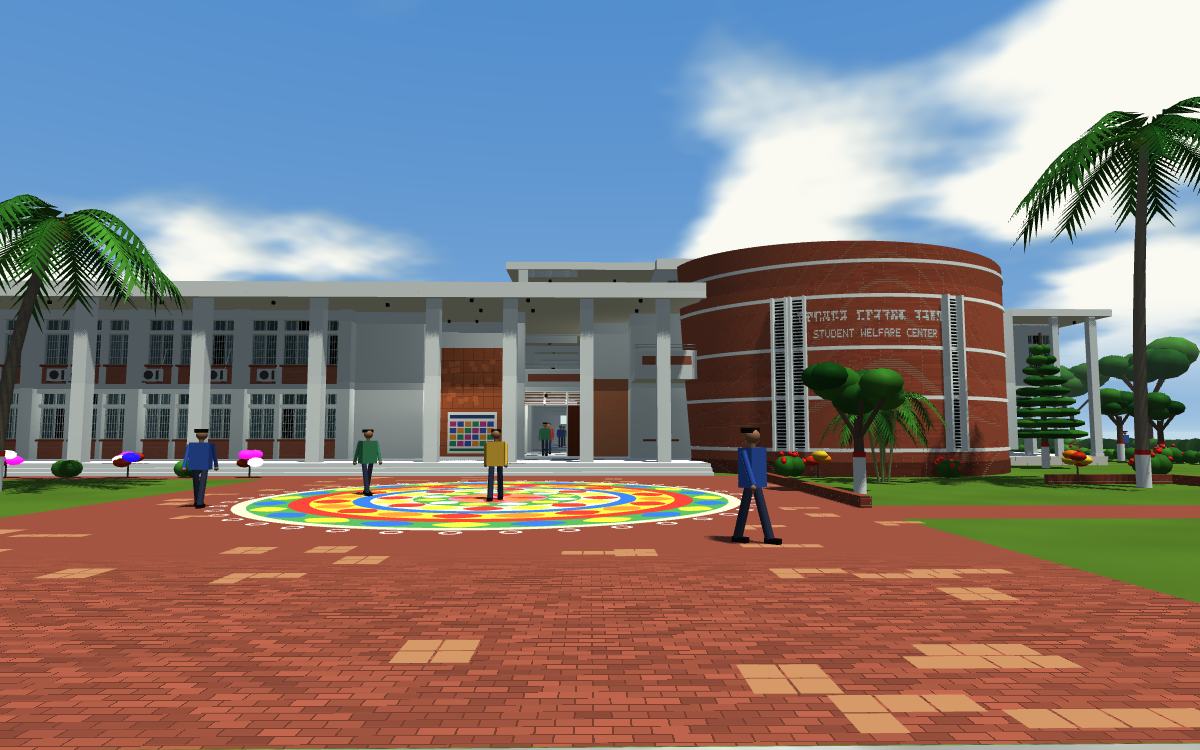
\includegraphics[width=0.86\textwidth]{main-entrance.png}\par
\vspace{1.0cm}
\begin{minipage}[t]{0.46\textwidth}
\raggedright
\textbf{Submitted by}\\[0.4em]
Abdullah Al Mahmud\\
Roll: 2107099\\
Department of CSE, KUET
\end{minipage}\hfill
\begin{minipage}[t]{0.46\textwidth}
\raggedright
\textbf{Course Teachers}\\[0.4em]
Mr.\ Md.\ Mubtashim Abrar Nihal\\[0.3em]
Mr.\ Md.\ Tajmilur Rahman
\end{minipage}
\vfill
{\large October 2026\par}
\end{titlepage}

% ---------------------------------------------------------------- abstract
\section*{Abstract}
This report describes an interactive three-dimensional model of the Student
Welfare Centre (SWC) of Khulna University of Engineering \& Technology. The
model was reconstructed from 93 photographs and is written in C++17 with
OpenGL~3.3. Every stage of the graphics pipeline is implemented in the
project itself: the geometric primitives, the vector and matrix mathematics,
the modelling, viewing and projection transformations, the Phong
illumination model, shadow mapping, procedural surface materials,
time-based animation, and first-person walking with collision detection. In
addition to the real-time renderer, the same scene can be rendered by a CPU
ray tracer that adds mirror reflections, exact shadows and ambient
occlusion. The finished scene contains about 367{,}000 triangles, 113 point
lights, 21 rotating fans, 7 moving vehicles and 35 walking pedestrians. The
report explains each feature together with the equations behind it, shows
the results, and states the limits of the work.

\vspace{0.3em}
\setcounter{tocdepth}{1}
\tableofcontents
\newpage

% ---------------------------------------------------------------- 1
\section{Introduction}
\subsection{Objective}
The aim of the project is to build a virtual 3D environment using the
techniques taught in the course, and to apply them to a real place. The
Student Welfare Centre was chosen because it combines regular architecture
(columns, window bays, corridors) with one distinctive form, a tall curved
brick wall, and because it could be photographed inside and outside.

No 3D model files, image textures or mathematics libraries are used. The
only external library is GLFW, which opens the window and reads the
keyboard and mouse.

\subsection{Requirements and how they are met}
\begin{table}[H]
\centering\small
\begin{tabularx}{\textwidth}{@{}rL{5.0cm}X@{}}
\toprule
\# & Requirement & Implementation \\
\midrule
1 & Virtual 3D environment & The SWC building, its interior, the site and the street behind it \\
2 & Objects from basic primitives & Nine canonical shapes; all geometry is assembled from them (Sec.~\ref{sec:prims}) \\
3 & Translation, rotation, scaling & Custom $4\times4$ matrices (Sec.~\ref{sec:transform}) \\
4 & Composite transformations & $T R S$ products, a transform stack, instanced moving objects (Sec.~\ref{sec:hier}) \\
5 & Custom vector and matrix operations & \code{Vec3}, \code{Mat4}, \code{Mat3}; dot, cross, product, inverse transpose \\
6 & Camera and viewing & Custom look-at matrix; orbit and walking cameras; 37 preset views (Sec.~\ref{sec:camera}) \\
7 & Perspective projection & Custom perspective and orthographic matrices \\
8 & Interactive manipulation & Mouse and keyboard camera; keys to move, rotate and scale the model \\
9 & Ambient, diffuse, specular light & One sun and 113 point lights (Sec.~\ref{sec:light}) \\
10 & Phong model, per-fragment & Evaluated in the fragment shader for every pixel \\
11 & Exploring from viewpoints & Preset views, orthographic elevations, walking mode (Sec.~\ref{sec:walk}) \\
\bottomrule
\end{tabularx}
\caption{Course requirements and their implementation.}
\end{table}

Features beyond the requirements are shadow mapping, procedural materials
and sky, transparent glass, animation of fans, traffic and people, collision
detection, and ray tracing.

% ---------------------------------------------------------------- 2
\section{System Overview}
\subsection{Structure of the program}
The source is divided into modules with one responsibility each
(Table~\ref{tab:modules}). The scene is built once at start-up into a
single array of vertices. A vertex holds eleven numbers: position, normal,
colour, a gloss value and a pattern number that selects a procedural
material. This array is uploaded to the graphics card once.

\begin{table}[H]
\centering\small
\begin{tabularx}{\textwidth}{@{}L{3.3cm}X@{}}
\toprule
Module & Responsibility \\
\midrule
\code{geometry/} & Vector and matrix mathematics; generators for the nine basic shapes; the vertex array and the transform stack \\
\code{scene/} & Materials and building dimensions; reusable parts (window bay, door, balcony panel); the building, interior, landscape, street, vehicles and people \\
\code{input/} & Orbit and walking cameras, preset views, keyboard and mouse handling \\
\code{navigation/} & Collision world for walking, and automatic route checks \\
\code{render/} & GLSL shaders, the OpenGL frame loop, the CPU ray tracer, image output \\
\code{tests/} & Unit tests for the shapes and for collision \\
\bottomrule
\end{tabularx}
\caption{Modules of the program.}\label{tab:modules}
\end{table}

\subsection{Rendering one frame}
Each frame is produced in the following order.
\begin{enumerate}
\item Read input; advance the fan angle and the clock for traffic and people.
\item \textbf{Shadow pass:} draw the scene from the sun's position, storing depth only.
\item Draw the procedural sky.
\item Select the 24 point lights nearest the camera.
\item \textbf{Opaque pass:} draw the static scene, then each fan, vehicle and person with its own model matrix.
\item \textbf{Transparent pass:} draw the glass panes sorted from far to near, with blending.
\end{enumerate}
The vertex array is laid out in ranges (static scene, one fan rotor, three
vehicle meshes, ten person meshes, the glass panes), so a moving object is
drawn by issuing one draw call for its range with a different matrix.

\begin{figure}[H]
\centering
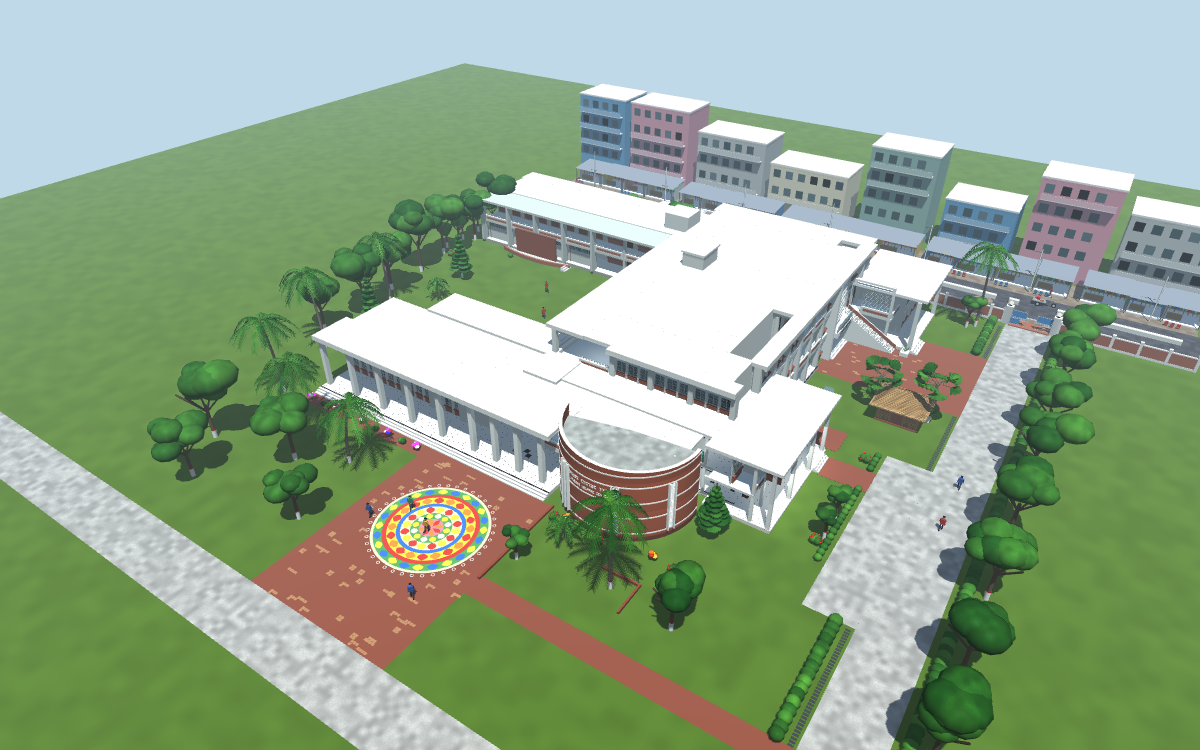
\includegraphics[width=0.64\textwidth]{aerial-overview.png}
\caption{Aerial view of the complete scene: the building around its courtyard,
the plaza, the campus roads, and the street with stalls behind.}
\end{figure}

% ---------------------------------------------------------------- 3
\section{Geometric Modelling}
\subsection{Primitives and triangle meshes}\label{sec:prims}
Everything drawn is a triangle. A four-sided face $(A,B,C,D)$ is split into
the triangles $(A,B,C)$ and $(A,C,D)$. Nine unit shapes are defined once and
then sized and placed: cube, cylinder, sphere, cone, frustum, open tube,
ring, plane and triangle (Fig.~\ref{fig:prims}).

\begin{figure}[H]
\centering
\begin{subfigure}[b]{0.46\textwidth}
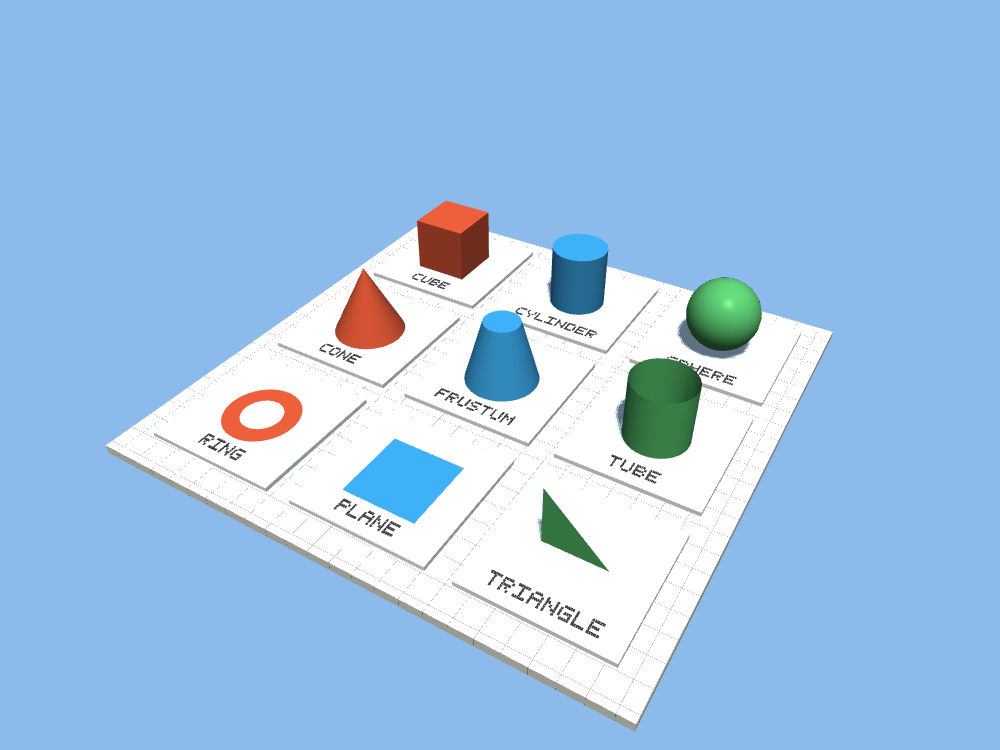
\includegraphics[width=\textwidth]{basic-objects.png}
\caption{The nine basic shapes.}\label{fig:prims}
\end{subfigure}\hfill
\begin{subfigure}[b]{0.46\textwidth}
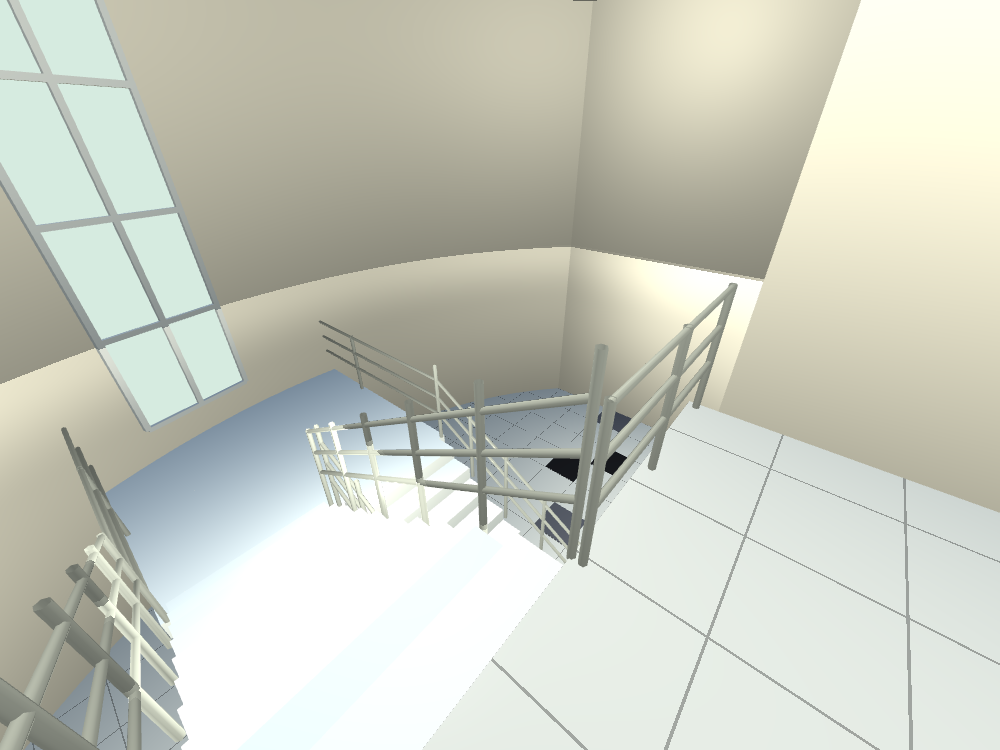
\includegraphics[width=\textwidth]{interior-oval-stair.png}
\caption{Curved stair built from ring sectors.}\label{fig:stair}
\end{subfigure}
\caption{Primitives, and a structure assembled from them.}
\end{figure}

\textbf{Cylinder.} With $N$ segments, $\theta_i = 2\pi i/N$, a point on the surface is
\begin{equation}
\vect p(\theta,y)=\bigl(c_x+r_x\cos\theta,\; y,\; c_z+r_z\sin\theta\bigr).
\end{equation}
Unequal radii $r_x\ne r_z$ give an elliptical cylinder.

\textbf{Cone and frustum.} The radius varies linearly with height,
$r(t)=(1-t)r_0+t\,r_1$ for $t\in[0,1]$; a cone has $r_1=0$.

\textbf{Sphere.} With latitude $\phi$ and longitude $\theta$,
\begin{equation}
\vect p=\vect c+r\,(\cos\phi\cos\theta,\;\sin\phi,\;\cos\phi\sin\theta).
\end{equation}
Scaling the axes unequally gives an ellipsoid, used for foliage.

\textbf{Rod.} A cylinder between two arbitrary points $A$ and $B$, used for
railings, branches and limbs. Its axis is $\hat{\vect a}=(B-A)/\lVert B-A\rVert$;
with any helper vector $\vect h$ not parallel to it,
$\vect u=\unit{\hat{\vect a}\times\vect h}$ and $\vect v=\hat{\vect a}\times\vect u$
span the circular cross-section.

\textbf{Curved wall.} The curved brick wall is a partial cylinder of
$60\times14$ flat quads. A point at angle $\theta$, height $y$ and radius $R$
about the centre $(c_x,c_z)$ is
\begin{equation}
\vect p=(c_x+R\sin\theta,\; y,\; c_z+R\cos\theta).
\end{equation}
Each vertex is given the true radial normal, so the lighting is smooth
although the surface is faceted.

\textbf{Curved stair.} The stair inside the curved wall follows it, so each
step is a sector of a ring between radii $r_{\mathrm{in}}=5.56$ and
$r_{\mathrm{out}}=7.02$ (Fig.~\ref{fig:stair}). For a tread depth $d_t=0.28$
on the middle radius $r_{\mathrm{mid}}=6.29$ and a riser $h_r=3.6/20=0.18$,
step $i$ spans
\begin{equation}
\Delta\theta=\frac{d_t}{r_{\mathrm{mid}}}\approx2.55^\circ,\qquad
\theta\in[\theta_0+i\,\Delta\theta,\;\theta_0+(i+1)\Delta\theta],\qquad
y_i=0.45+(i+1)\,h_r .
\end{equation}
Twenty steps turn through about $51^\circ$ and rise one storey.

\subsection{Vectors and matrices}
All mathematics is written in the project. For vectors $\vect a,\vect b$:
\begin{equation}
\vect a\cdot\vect b=a_xb_x+a_yb_y+a_zb_z,\qquad
\vect a\times\vect b=(a_yb_z-a_zb_y,\;a_zb_x-a_xb_z,\;a_xb_y-a_yb_x).
\end{equation}
The dot product measures how closely two directions agree and drives all
lighting. Writing $\unit{\vect a}=\vect a/\lVert\vect a\rVert$ for a vector scaled to length one, the cross product gives a perpendicular vector; the normal of a
flat triangle is $\vect n=\unit{(B-A)\times(C-A)}$. Matrices are $4\times4$
and multiply as $(AB)_{ij}=\sum_{k}A_{ik}B_{kj}$.

\subsection{Transformations}\label{sec:transform}
A point is written in homogeneous form $(x,y,z,1)^T$ so that translation
becomes a matrix:
\begin{equation}
T=\begin{bmatrix}1&0&0&t_x\\0&1&0&t_y\\0&0&1&t_z\\0&0&0&1\end{bmatrix},\quad
S=\begin{bmatrix}s_x&0&0&0\\0&s_y&0&0\\0&0&s_z&0\\0&0&0&1\end{bmatrix},\quad
R_y(\theta)=\begin{bmatrix}\cos\theta&0&\sin\theta&0\\0&1&0&0\\-\sin\theta&0&\cos\theta&0\\0&0&0&1\end{bmatrix}.
\end{equation}
A rotation about the X axis, $R_x$, is defined in the same way and is used,
for example, to turn a cylinder on its side to make a wheel.

\textbf{Composite transformation.} An object is placed with
\begin{equation}
M = T\,R_y\,S ,
\end{equation}
which scales first, then rotates, then translates. The order matters:
translating before rotating would swing the object around the origin.

\textbf{Normals.} Under non-uniform scaling a normal transformed by $M$ is no
longer perpendicular to the surface. With $A$ the upper-left $3\times3$ part
of $M$, normals are transformed by the inverse transpose:
\begin{equation}
\vect n'=\unit{(A^{-1})^{T}\vect n}.
\end{equation}

\subsection{Hierarchy and instancing}\label{sec:hier}
\textbf{Transform stack.} A small class \code{Place} multiplies the current
matrix by a local one and restores it when its scope ends:
\begin{equation}
M_{\mathrm{child}}=M_{\mathrm{parent}}\,M_{\mathrm{local}}.
\end{equation}
A window bay is therefore written once in its own coordinates, placed
repeatedly along a wing, and the wing is placed on the site. The cafeteria
front is modelled facing $+Z$ and a single \code{Place} turns it to face the road.

\textbf{Instancing.} One mesh is drawn many times with different matrices
(Table~\ref{tab:inst}). This is how 21 fans, 7 vehicles and 35 people are
drawn from only 14 small meshes.

\begin{table}[H]
\centering\small
\begin{tabular}{@{}lll@{}}
\toprule
Mesh & Instances & Model matrix \\
\midrule
Fan rotor & 21 & $M_{\mathrm{scene}}\,T(\vect h_k)\,R_y(\theta(t))$ \\
Easybike, cycle-van, bus & 7 & $M_{\mathrm{scene}}\,T(x(t),\,0.03,\,z_l)\,R_y(0\ \text{or}\ \pi)$ \\
Person (5 colours $\times$ 2 poses) & 35 & $M_{\mathrm{scene}}\,T(\vect p(t))\,R_y(\psi)$ \\
\bottomrule
\end{tabular}
\caption{Instanced objects and their composite transformations.}\label{tab:inst}
\end{table}

\subsection{The modelled spaces}
The model follows the photographs space by space. Outside: the plaza with a
circular \emph{alpona} built from rings and petal shapes, the front
colonnade and portico, the curved wall with pale bands, louvre strips and
lettering that follows the curve, the courtyard with its stage, the
cafeteria front with an external stair, and the shop wing. Inside: the
entrance lobby with a terracotta relief wall, an indoor-games hall, the
Shwapno shop, a cafeteria dining hall whose corridor wall is glass, tiled
corridors with black accent tiles, two stairs, and a first-floor terrace
under white portal frames. Behind the building: a boundary wall with two
gates, a road with a central divider, and a row of stalls.

\begin{figure}[H]
\centering
\begin{subfigure}[b]{0.325\textwidth}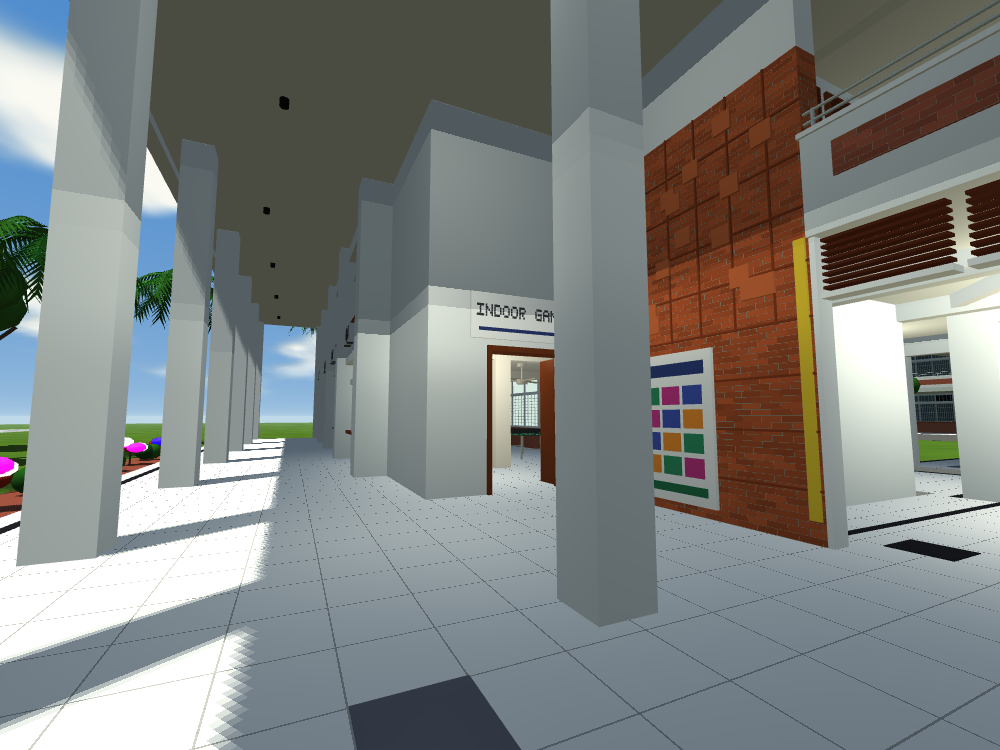
\includegraphics[width=\textwidth]{interior-lobby.png}\caption{Entrance lobby}\end{subfigure}\hfill
\begin{subfigure}[b]{0.325\textwidth}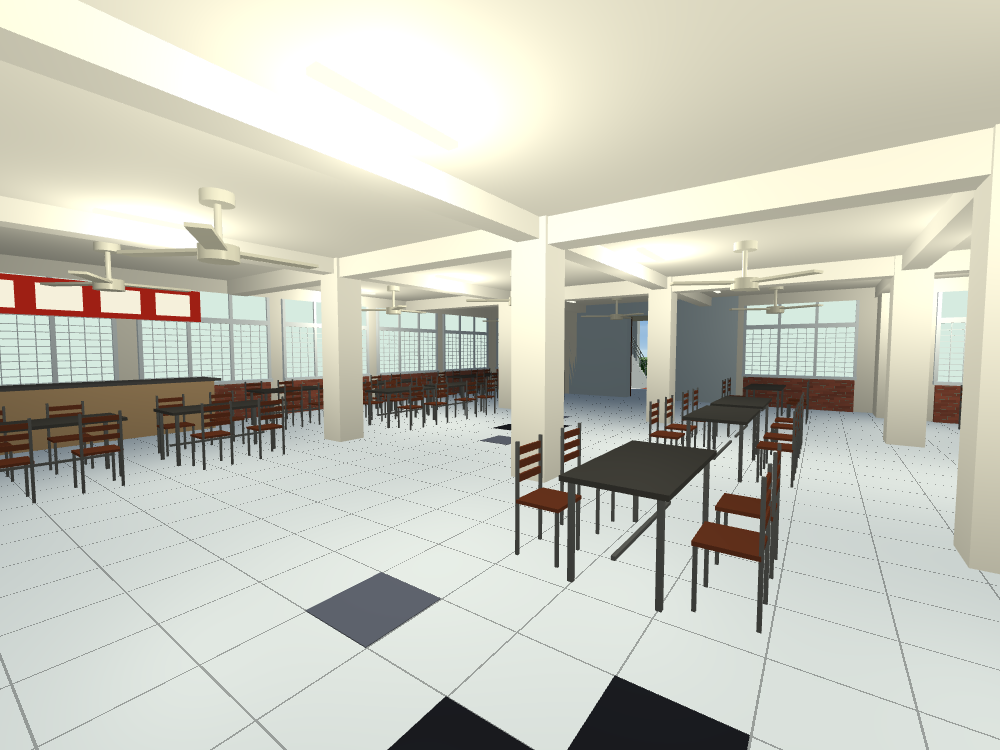
\includegraphics[width=\textwidth]{interior-cafeteria-hall.png}\caption{Cafeteria hall}\end{subfigure}\hfill
\begin{subfigure}[b]{0.325\textwidth}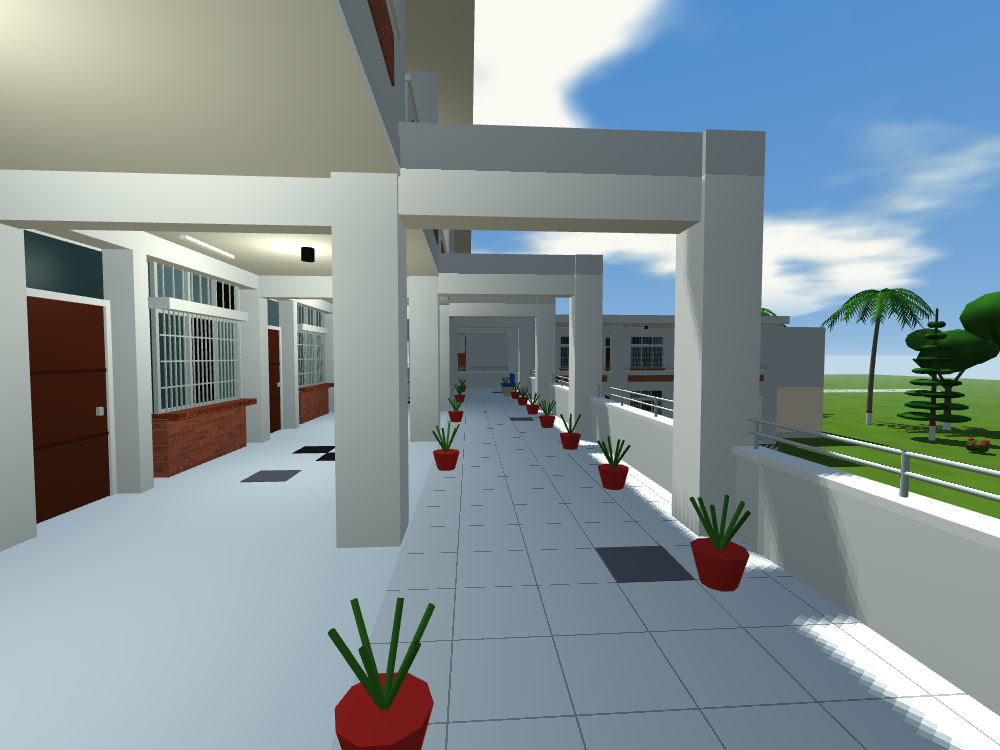
\includegraphics[width=\textwidth]{interior-terrace.png}\caption{First-floor terrace}\end{subfigure}\\[4pt]
\begin{subfigure}[b]{0.325\textwidth}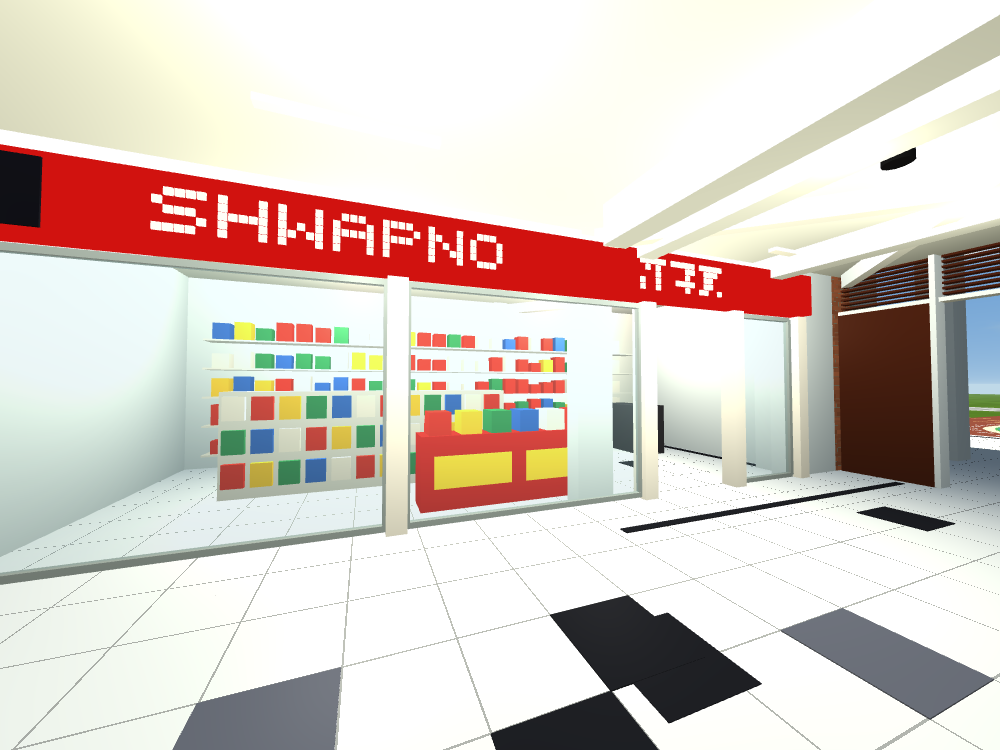
\includegraphics[width=\textwidth]{interior-shop-hall.png}\caption{Shwapno shop}\end{subfigure}\hfill
\begin{subfigure}[b]{0.325\textwidth}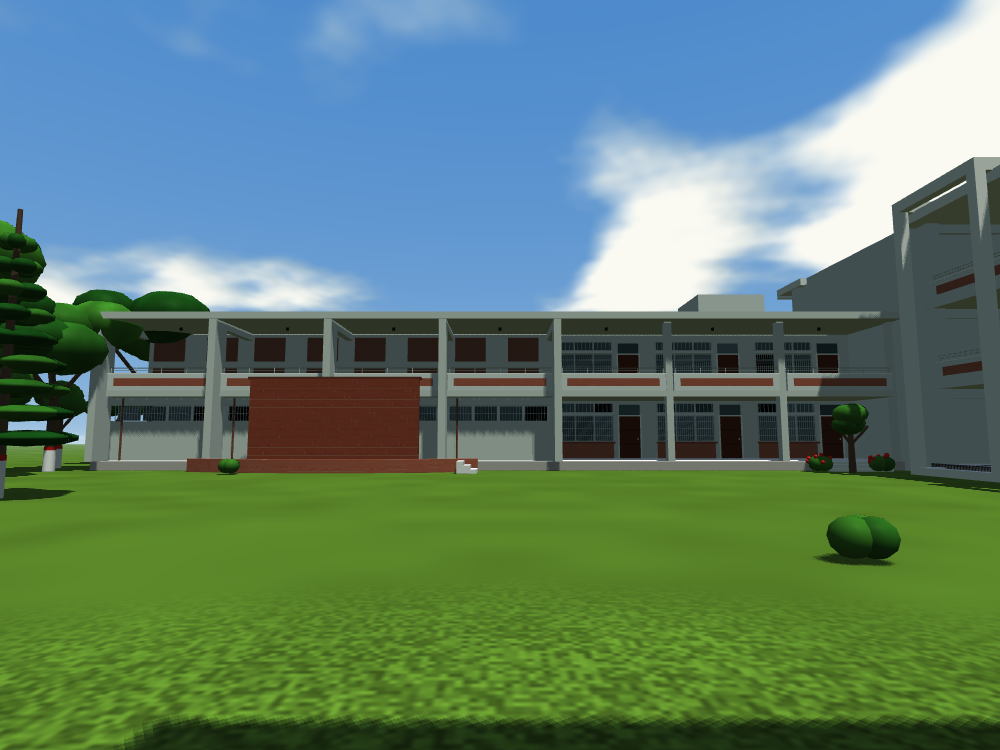
\includegraphics[width=\textwidth]{courtyard-stage.png}\caption{Courtyard and stage}\end{subfigure}\hfill
\begin{subfigure}[b]{0.325\textwidth}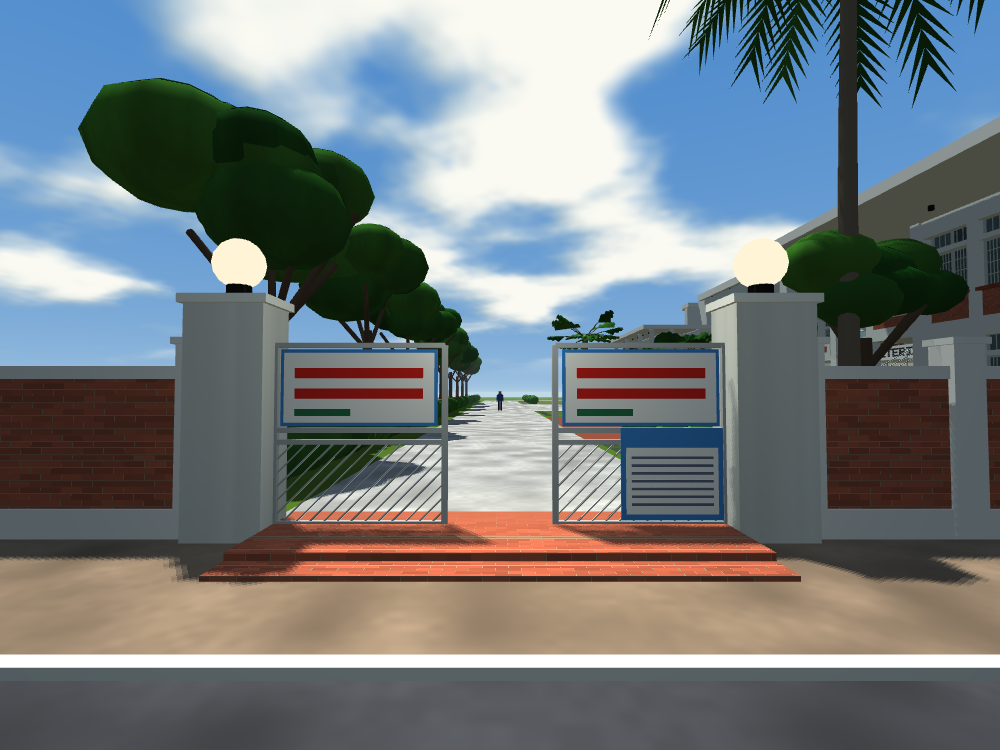
\includegraphics[width=\textwidth]{street-gate.png}\caption{Campus gate}\end{subfigure}
\caption{Some of the modelled spaces, rendered in real time.}
\end{figure}

% ---------------------------------------------------------------- 4
\section{Viewing and Projection}\label{sec:camera}
\subsection{Orbit camera}
The camera circles a target $\vect c$ at distance $d$ with yaw $\psi$ and
pitch $\phi$. Its eye position lies on a sphere:
\begin{equation}
\vect e=\vect c+d\,(\cos\phi\sin\psi,\;\sin\phi,\;\cos\phi\cos\psi).
\end{equation}
Dragging the mouse changes $\psi$ and $\phi$; the wheel multiplies $d$ by
$0.9$ per notch.

\subsection{View matrix}
The look-at matrix is built from the eye, the target and an up hint $\vect u_0$:
\begin{equation}
\vect f=\unit{\vect c-\vect e},\qquad
\vect s=\unit{\vect f\times\vect u_0},\qquad
\vect u=\vect s\times\vect f,
\end{equation}
\begin{equation}
V=\begin{bmatrix}
s_x&s_y&s_z&-\vect s\cdot\vect e\\
u_x&u_y&u_z&-\vect u\cdot\vect e\\
-f_x&-f_y&-f_z&\vect f\cdot\vect e\\
0&0&0&1\end{bmatrix}.
\end{equation}
$V$ moves the world so that the eye is at the origin looking along $-Z$.

\subsection{Projection}
For a vertical field of view $\alpha$, aspect ratio $a$, near and far
distances $n,f$, and $q=1/\tan(\alpha/2)$, the perspective matrix is
\begin{equation}
P=\begin{bmatrix}
q/a&0&0&0\\0&q&0&0\\
0&0&-\dfrac{f+n}{f-n}&-\dfrac{2fn}{f-n}\\
0&0&-1&0\end{bmatrix}.
\end{equation}
The last row copies depth into $w$; the division by $w$ that follows makes
distant objects smaller. The complete chain for a vertex is
\begin{equation}
\vect p_{\mathrm{clip}}=P\,V\,M\,\vect p,\qquad
\vect p_{\mathrm{ndc}}=\vect p_{\mathrm{clip},xyz}/p_{\mathrm{clip},w}.
\end{equation}
An orthographic matrix, which has no division by depth, is used for the
architectural elevations and plan (Fig.~\ref{fig:ortho}) and for the sun's
shadow camera.

\begin{figure}[H]
\centering
\begin{subfigure}[b]{0.40\textwidth}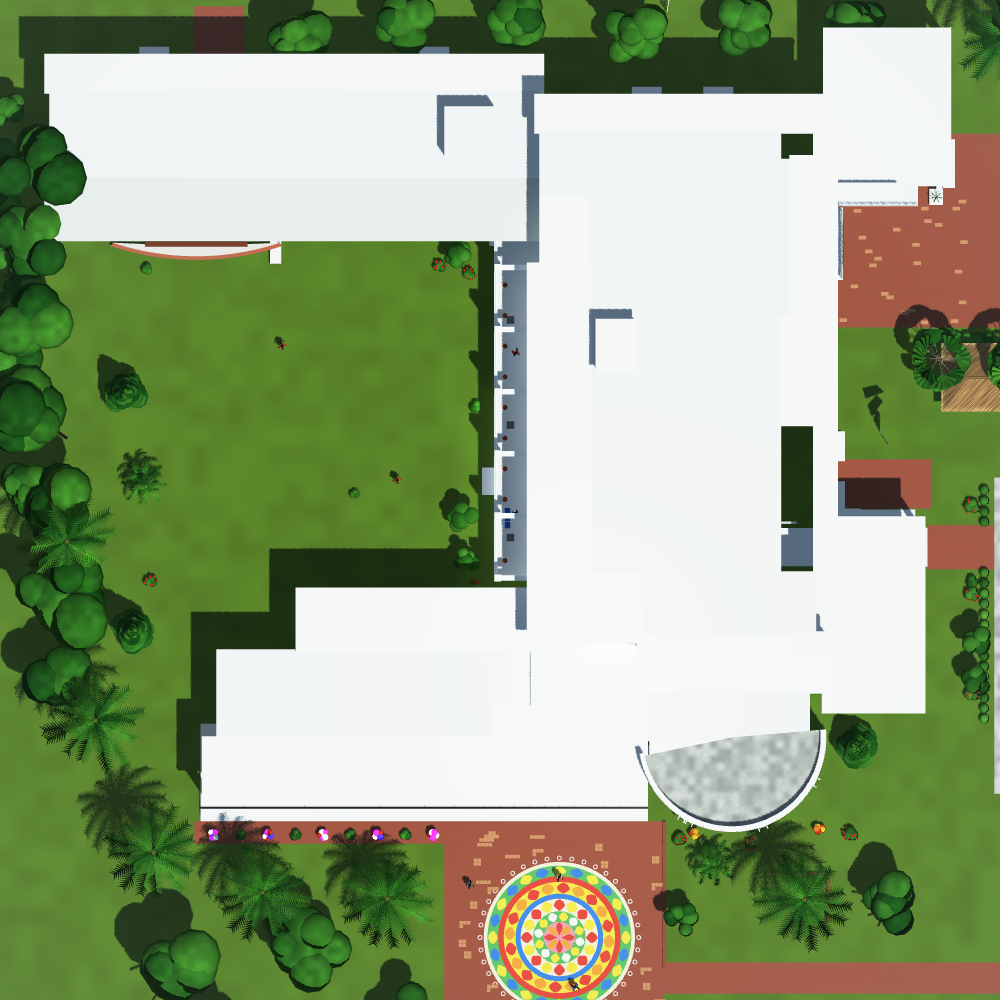
\includegraphics[width=\textwidth]{orthographic-plan.png}\caption{Orthographic plan}\label{fig:ortho}\end{subfigure}\hfill
\begin{subfigure}[b]{0.56\textwidth}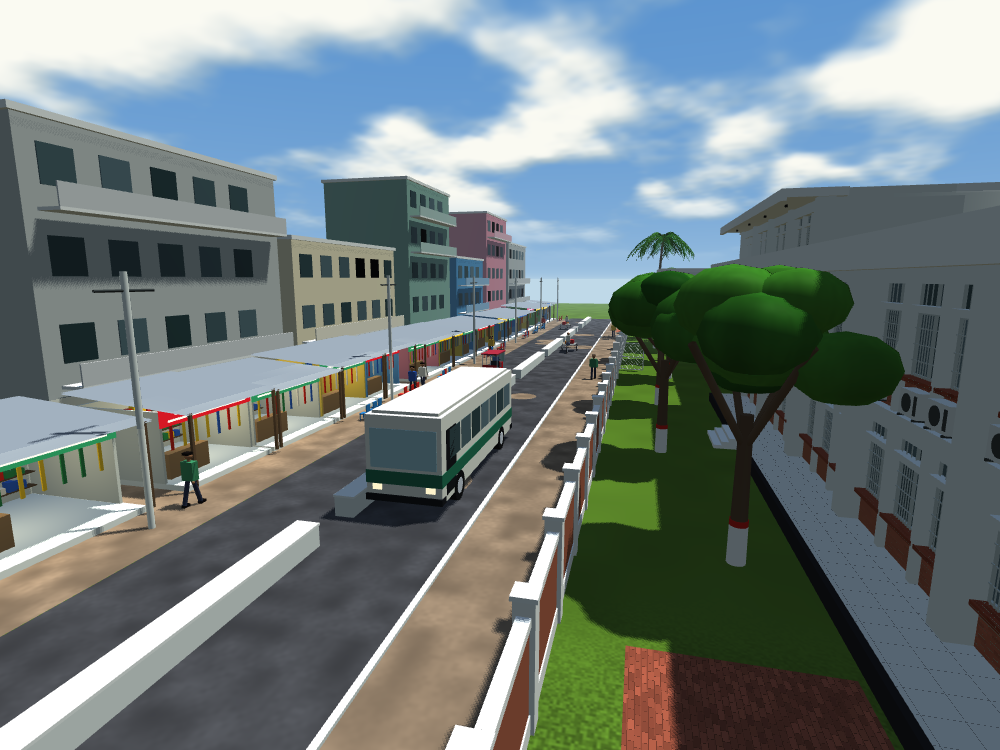
\includegraphics[width=\textwidth]{street-traffic.png}\caption{Perspective view of the street}\end{subfigure}
\caption{The two projections. In (a) size is independent of distance; in (b) it is not.}
\end{figure}

% ---------------------------------------------------------------- 5
\section{Illumination and Shading}\label{sec:light}
\subsection{Phong illumination, per fragment}
Lighting is computed for every pixel in the fragment shader, using the
normal interpolated across the triangle. Let $\vect n$ be the normal,
$\vect l$ the direction to the sun, $\vect v$ the direction to the eye, $g$
the gloss of the material and $S_h\in[0,1]$ the shadow factor.
\begin{align}
\text{Diffuse:}\quad & D=\max(\vect n\cdot\vect l,0)\,S_h,\\
\text{Specular:}\quad & \vect r=2(\vect n\cdot\vect l)\vect n-\vect l,\qquad
k=8+88g,\qquad H=\max(\vect v\cdot\vect r,0)^{k}\,g\,S_h,\\
\text{Ambient:}\quad & \vect A=0.62\,\operatorname{mix}\bigl(\vect C_{\mathrm{ground}},\vect C_{\mathrm{sky}},\tfrac12 n_y+\tfrac12\bigr).
\end{align}
The final colour is
\begin{equation}
\vect C=\vect C_{\mathrm{base}}\odot\bigl(\vect A+0.95\,\vect C_{\mathrm{sun}}D+\vect L_d\bigr)
+0.6\,\vect C_{\mathrm{sun}}H+0.5\,g\,\vect L_s ,
\end{equation}
where $\odot$ is component-wise multiplication and $\vect L_d,\vect L_s$ are
the point-light sums defined below. The ambient term stands for light
arriving from all directions: upward-facing surfaces take the colour of the
sky and downward-facing ones the colour of the ground. A higher gloss gives
a smaller, sharper highlight.

\subsection{Point lights and emission}
Sunlight does not reach the corridors and halls, so every ceiling fixture
and stall lamp is a point light at $\vect p_i$ with colour $\vect c_i$ and
radius $r_i$. For a surface point $\vect p$, with $d_i=\lVert\vect p_i-\vect p\rVert$
and $\vect l_i=(\vect p_i-\vect p)/d_i$, the attenuation is
\begin{equation}
a_i=s_i\,\frac{\bigl(1-(d_i/r_i)^4\bigr)^{2}}{1+0.22\,d_i+0.20\,d_i^{2}} .
\end{equation}
The denominator is the usual constant--linear--quadratic falloff. The
numerator brings the light smoothly to zero at its radius, and $s_i$ fades
it out one storey below the fixture so that a lamp lights only its own floor.
\begin{equation}
\vect L_d=\sum_i\vect c_i\,a_i\bigl(0.25+0.75\max(\vect n\cdot\vect l_i,0)\bigr),\qquad
\vect L_s=\sum_i\vect c_i\,a_i\max(\vect v\cdot\vect r_i,0)^{k}.
\end{equation}
The constant $0.25$ stands in for light bounced from white walls. Lamps,
fluorescent tubes, lit signs and window glazing seen from indoors are
\emph{emissive}: they output their own colour regardless of the lighting.

\subsection{Shadow mapping}
The scene is first drawn from the sun's position with an orthographic
camera into a $4096\times4096$ depth texture. When a pixel is shaded, its
world position is transformed into the sun's view; if it is farther from
the sun than the stored depth, something lies in front of it and it is in
shadow:
\begin{equation}
\vect p_L=P_LV_L\,(\vect p+0.05\,\hat{\vect n}),\qquad
\vect q=\tfrac12\,\vect p_{L,xyz}/p_{L,w}+\tfrac12 .
\end{equation}
A bias $\beta=0.0006+0.0012\,(1-\max(\vect n\cdot\vect l,0))$ prevents a
surface from shadowing itself. Nine neighbouring texels are tested and
averaged (percentage-closer filtering), which softens the shadow edge:
\begin{equation}
S_h=\frac19\sum_{i=-1}^{1}\sum_{j=-1}^{1}
\Bigl[\,q_z-\beta\le D_{\mathrm{map}}\bigl(q_x+\tfrac{i}{4096},\,q_y+\tfrac{j}{4096}\bigr)\Bigr].
\end{equation}
Fans, vehicles and people are drawn into the shadow map as well, so their
shadows move with them.

\subsection{Procedural materials}
No image textures are used. The pattern number of a vertex selects a
function of world position in the shader. For brick and paving, laid in
running bond with units of size $(w,h)$ at surface coordinates $(u,v)$:
\begin{equation}
j=\lfloor v/h\rfloor,\qquad
\vect c=\bigl(u/w+\tfrac12(j\bmod2),\;v/h\bigr).
\end{equation}
The fractional part of $\vect c$ locates the pixel within its brick (near
zero it is mortar); the integer part identifies the brick and seeds a hash
that varies its colour. Floor tiles use the same idea on a straight
$0.6$\,m grid. Grass, bark and thatch use value noise: random values on a
grid blended with the weight $w(t)=t^{2}(3-2t)$. When a pattern becomes
smaller than a pixel it is faded to its average colour, which removes
shimmering. The sky blends from horizon to zenith and adds clouds from five
octaves of noise; distant surfaces are fogged by
$F=1-e^{-0.006\max(d-45,\,0)}$.

\subsection{Transparent glass}
Glass panes are drawn after all opaque geometry, sorted from far to near,
with depth writing switched off:
\begin{equation}
\vect C_{\mathrm{out}}=\alpha\,\vect C_{\mathrm{glass}}+(1-\alpha)\,\vect C_{\mathrm{behind}},\qquad\alpha=0.20 .
\end{equation}
Glass also reflects more strongly at grazing angles,
$F_g=0.08+0.62\,(1-\max(\vect n\cdot\vect v,0))^{3}$.

% ---------------------------------------------------------------- 6
\section{Animation}
All motion is driven by elapsed time, capped at $0.05$\,s per frame so that
a pause does not cause a jump. Pressing \code{P} freezes all of it.

\subsection{Ceiling fans}
\begin{equation}
\theta\leftarrow(\theta+\omega\,\Delta t)\bmod2\pi,\qquad\omega=240^\circ/\mathrm{s}.
\end{equation}
The mount is static; only the rotor is drawn with $T(\vect h_k)\,R_y(\theta)$.

\subsection{Road traffic}
Four easybikes, two cycle-vans and one bus use the road behind the building
(Fig.~\ref{fig:traffic}). A vehicle with speed $v$, offset $s_0$ and loop
length $L$ has travelled
\begin{equation}
s(t)=(s_0+vt)\bmod L
\end{equation}
round its loop. Only the first $D=116$\,m of the loop lies on the road, so
the vehicle is drawn while $s\le D$, at $x=x_{\mathrm{start}}+s$ in one lane
and $x=x_{\mathrm{end}}-s$ in the other. Traffic keeps to the left of the
divider. Vehicles in a lane share $v$ and $L$, so their spacing is constant
and they never overlap. The bus is visible for $D/L\approx32\%$ of the
time, which makes it an occasional sight.

\begin{figure}[H]
\centering
\begin{subfigure}[b]{0.325\textwidth}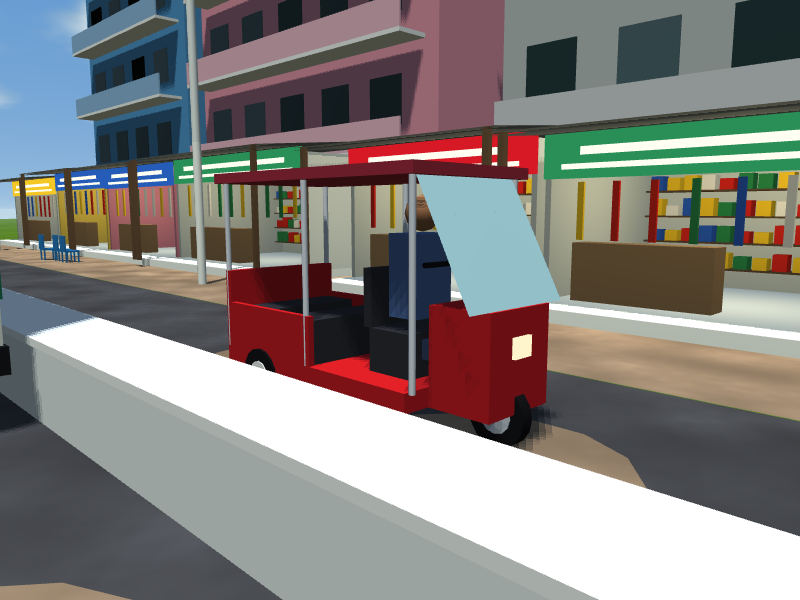
\includegraphics[width=\textwidth]{traffic-easybike.png}\caption{Easybike}\end{subfigure}\hfill
\begin{subfigure}[b]{0.325\textwidth}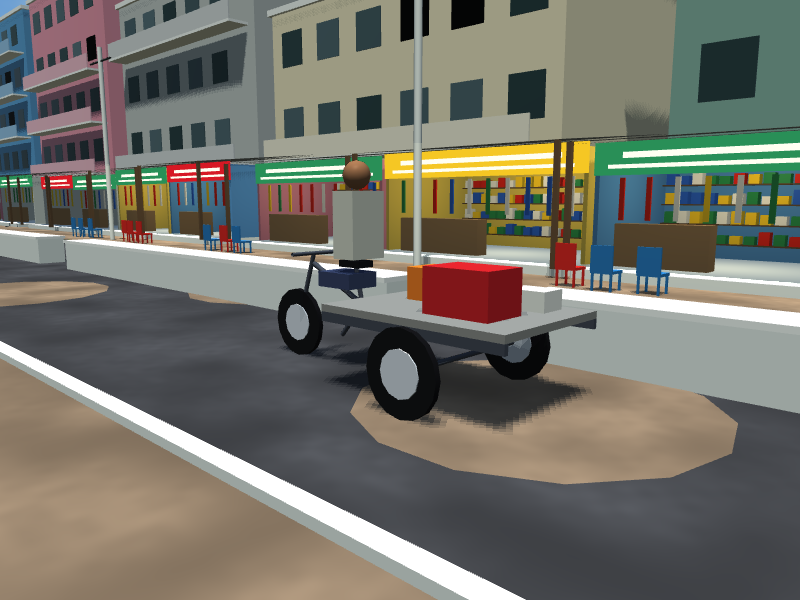
\includegraphics[width=\textwidth]{traffic-van.png}\caption{Cycle-van}\end{subfigure}\hfill
\begin{subfigure}[b]{0.325\textwidth}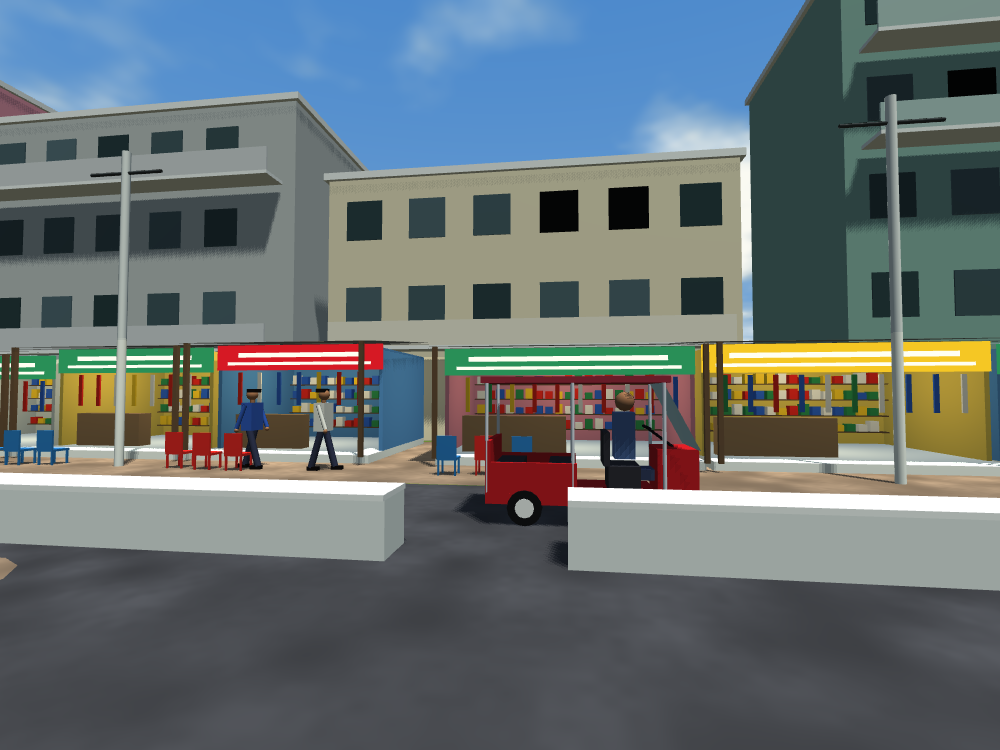
\includegraphics[width=\textwidth]{street-stalls.png}\caption{Stalls across the road}\end{subfigure}
\caption{The street behind the SWC, with moving vehicles.}\label{fig:traffic}
\end{figure}

\subsection{Pedestrians}
Thirty-five people walk fourteen routes inside and outside the building. A
route is a polyline $\vect w_0,\dots,\vect w_n$ of total length $L$. The
distance of a walker along it is
\begin{equation}
s(t)=\begin{cases}
(s_0+vt)\bmod L & \text{closed loop},\\[2pt]
L-\bigl|\,(s_0+vt)\bmod 2L-L\,\bigr| & \text{open route (there and back)}.
\end{cases}
\end{equation}
On the segment that contains $s$, at fraction $u$ along it and with travel
direction $\vect d$, the position and heading are
\begin{equation}
\vect p=(1-u)\,\vect w_i+u\,\vect w_{i+1},\qquad
\psi=\operatorname{atan2}(-d_z,\;d_x).
\end{equation}
Because $\vect p$ is interpolated in all three coordinates, a route that
climbs the entrance steps lifts the walker with it. Two meshes with opposite
legs forward alternate about twice a second to suggest a stride.

% ---------------------------------------------------------------- 7
\section{Walking and Collision Detection}\label{sec:walk}
In walking mode the viewer moves through the model at eye height. Collision
uses the same triangles that are drawn, so what is seen is what blocks.

\textbf{Spatial grid.} Triangles are stored in $2$\,m cells indexed by
$(\lfloor x/2\rfloor,\lfloor z/2\rfloor)$, so each step tests only nearby ones.

\textbf{Movement.} The walker is a cylinder of radius $0.18$ and height
$1.78$ with eyes at $1.6$. From forward input $f$, sideways input $r$ and yaw $\psi$,
\begin{equation}
\vect d=(r\cos\psi-f\sin\psi,\;0,\;-r\sin\psi-f\cos\psi),\qquad
\Delta\vect p=\hat{\vect d}\,v\,\Delta t ,
\end{equation}
with $v=2.4$\,m/s. Normalising $\vect d$ prevents diagonal movement from
being faster. Each step is divided into pieces of at most $0.06$ so that a
thin wall cannot be skipped.

\textbf{Finding the floor.} For a nearly horizontal triangle $ABC$ the
barycentric coordinates of the walker in plan are found from
\begin{equation}
\begin{bmatrix}B_x-A_x&C_x-A_x\\B_z-A_z&C_z-A_z\end{bmatrix}
\begin{bmatrix}u\\v\end{bmatrix}=
\begin{bmatrix}x-A_x\\z-A_z\end{bmatrix},\qquad
y=A_y+u\,(B_y-A_y)+v\,(C_y-A_y).
\end{equation}
The walker is over the triangle when $u\ge0$, $v\ge0$ and $u+v\le1$. A
floor up to $0.24$ higher can be stepped onto, which is how stairs are
climbed. If no floor is found the move is refused, so the walker cannot
leave a balcony.

\textbf{Obstacles.} Other triangles are clipped to the height range of the
body and projected to plan. The closest point on an edge $AB$ to the
walker's centre $P$ is
\begin{equation}
t=\operatorname{clamp}\!\left(\frac{(P-A)\cdot(B-A)}{\lVert B-A\rVert^{2}},0,1\right),\qquad
Q=A+t\,(B-A),
\end{equation}
and the move is blocked if $\lVert P-Q\rVert$ is less than the body radius.
When a move is blocked its X and Z parts are tried separately, so the walker
slides along a wall instead of stopping.

% ---------------------------------------------------------------- 8
\section{Ray Tracing}
A second renderer traces rays through the same triangles, materials, lights
and camera, entirely on the CPU. It produces effects that the Phong
rasteriser cannot (Fig.~\ref{fig:rt}).

\begin{figure}[H]
\centering
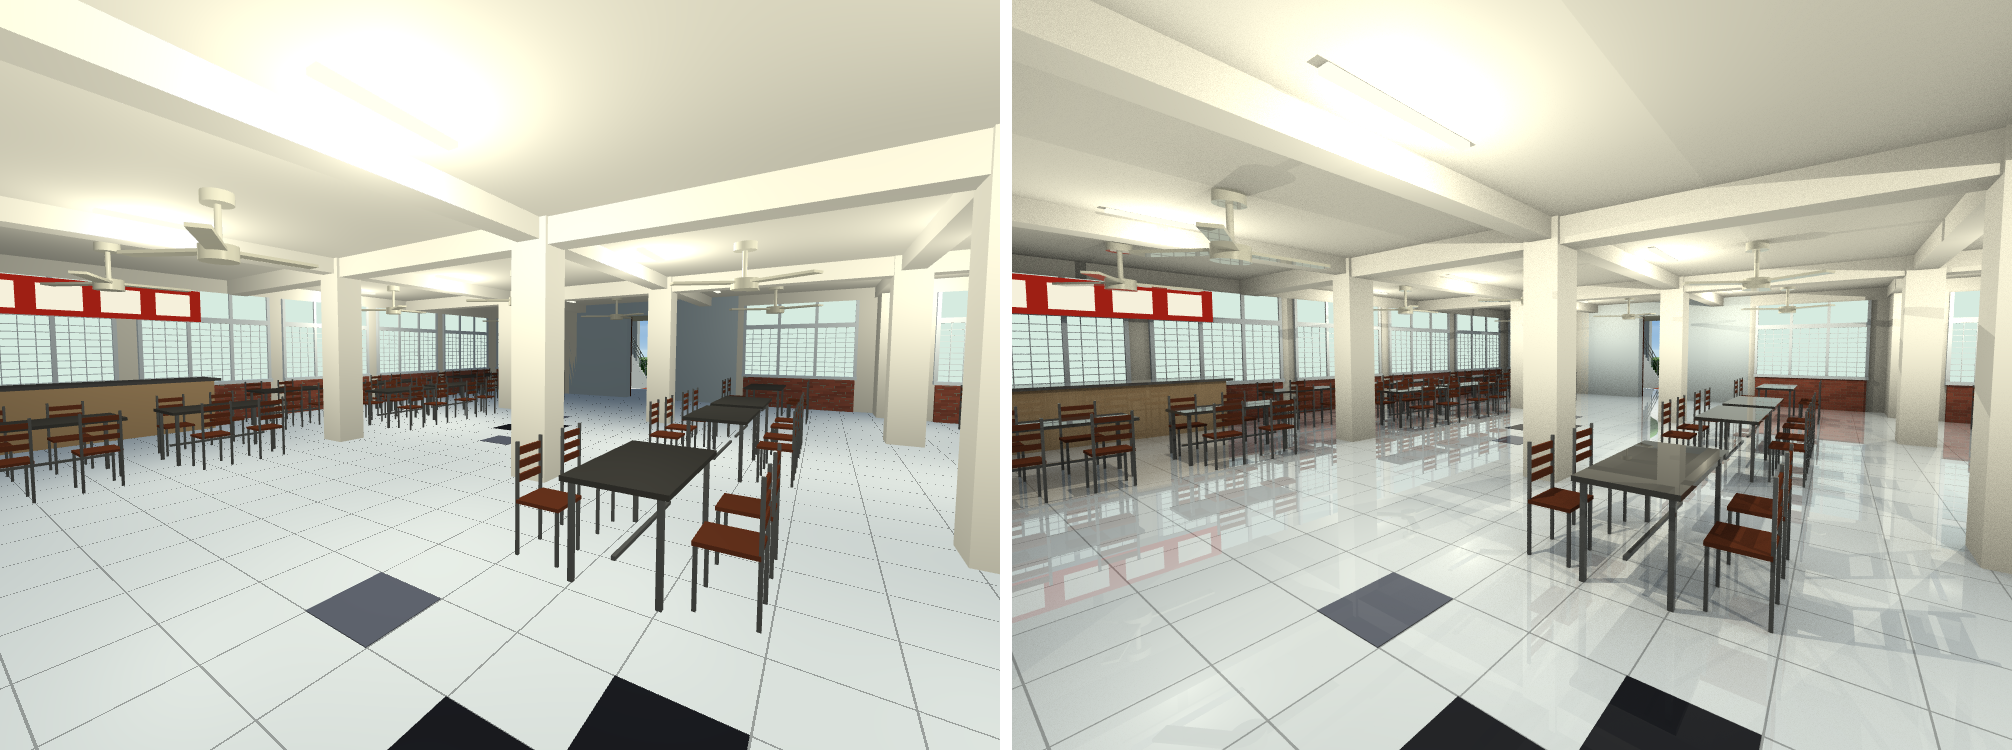
\includegraphics[width=\textwidth]{raster-vs-raytraced.png}
\caption{The cafeteria hall from one camera position. Left: real-time
OpenGL. Right: ray traced. The ray tracer adds the reflection of windows and
furniture in the polished floor, a shadow from every lamp, and darkening
where surfaces meet.}\label{fig:rt}
\end{figure}

\subsection{Primary rays}
Ray generation is projection run in reverse: the rasteriser maps points to
pixels, the ray tracer maps pixels to directions. For a sample at
$(p_x,p_y)$ in a $W\times H$ image, with the camera axes
$\vect f,\vect s,\vect u$ of Section~\ref{sec:camera},
\begin{equation}
x_n=\frac{2p_x}{W}-1,\quad y_n=1-\frac{2p_y}{H},\qquad
\vect d=\unit{\vect f+x_n\,a\tan\tfrac{\alpha}{2}\,\vect s+y_n\tan\tfrac{\alpha}{2}\,\vect u}.
\end{equation}
Points on the ray are $\vect o+t\,\vect d$.

\subsection{Ray--triangle intersection}
The M\"oller--Trumbore method is used. A triangle with corner $\vect p_0$
and edges $\vect e_1,\vect e_2$ contains the points
$\vect p_0+u\,\vect e_1+v\,\vect e_2$. Equating this with the ray and
solving by Cramer's rule, with $\vect s=\vect o-\vect p_0$:
\begin{equation}
\vect h=\vect d\times\vect e_2,\quad\vect q=\vect s\times\vect e_1,\quad
\Delta=\vect e_1\cdot\vect h,\qquad
u=\frac{\vect s\cdot\vect h}{\Delta},\quad
v=\frac{\vect d\cdot\vect q}{\Delta},\quad
t=\frac{\vect e_2\cdot\vect q}{\Delta}.
\end{equation}
The ray hits when $u\ge0$, $v\ge0$, $u+v\le1$ and $t>0$. The same $u,v$
interpolate the vertex normals.

\subsection{Bounding-volume hierarchy}
Testing 350{,}000 triangles for every ray is impractical, so the triangles
are grouped into a binary tree of axis-aligned boxes. A ray that misses a
box skips everything in it. The ray meets a box when its three slab
intervals overlap:
\begin{equation}
t_{\mathrm{in}}=\max_k\min\!\left(\tfrac{b^{\min}_k-o_k}{d_k},\tfrac{b^{\max}_k-o_k}{d_k}\right),\quad
t_{\mathrm{out}}=\min_k\max\!\left(\tfrac{b^{\min}_k-o_k}{d_k},\tfrac{b^{\max}_k-o_k}{d_k}\right),\quad
t_{\mathrm{out}}\ge\max(t_{\mathrm{in}},0).
\end{equation}
The tree is built with the surface-area heuristic: twelve candidate splits
along the longest axis are compared and the one with the lowest cost
$A_LN_L+A_RN_R$ is chosen, where $A$ is the surface area of a child box and
$N$ its triangle count. The area of a box is proportional to the chance
that a random ray hits it, so the cost estimates the work that remains.

\subsection{Shadows, reflection and transmission}
\textbf{Shadow rays.} From each hit point a ray is sent to the sun and to
each nearby lamp; the light contributes only if the ray is unobstructed.
The resulting shadows are exact, and every lamp casts them.

\textbf{Reflection.} For polished surfaces the ray is mirrored,
$\vect d_r=\vect d-2(\vect d\cdot\vect n)\vect n$, and traced again, up to
three bounces. The fraction reflected follows Schlick's approximation of
the Fresnel equations:
\begin{equation}
F=F_0+(1-F_0)(1-\cos\theta)^{5},\qquad
\vect C=(1-F)\,\vect C_{\mathrm{local}}+F\,\vect C(\vect d_r).
\end{equation}
A floor seen from above reflects a few per cent; seen at a grazing angle it
is almost a mirror, as it is in the photographs.

\textbf{Glass.} A thin flat pane refracts a ray on entry and refracts it
back on exit, so the ray leaves in its original direction. The tracer
therefore continues the ray and keeps $20\%$ of the pane's own colour,
matching the blend of the rasteriser.

\subsection{Ambient occlusion and anti-aliasing}
Eight short rays are sent over the hemisphere above each visible point and
the ambient term is reduced by the fraction that are blocked,
$\vect A'=\vect A\,(1-0.70\,N_{\mathrm{blocked}}/N)$. Directions are
cosine-weighted: from random numbers $\xi_1,\xi_2$,
\begin{equation}
\boldsymbol\omega=\sqrt{\xi_1}\cos(2\pi\xi_2)\,\vect t
+\sqrt{\xi_1}\sin(2\pi\xi_2)\,\vect b+\sqrt{1-\xi_1}\,\vect n .
\end{equation}
Each pixel is divided into a $g\times g$ grid with one jittered sample per
cell, and the results are averaged. Image rows are rendered in parallel by
one thread per processor.

\begin{table}[H]
\centering\small
\begin{tabular}{@{}lll@{}}
\toprule
 & Rasteriser & Ray tracer \\
\midrule
Visibility & Depth buffer & Nearest hit in the hierarchy \\
Sun shadows & Shadow map, $3\times3$ filter & Shadow ray, exact \\
Lamp shadows & None & One shadow ray per lamp \\
Reflections & Estimated, glass only & Traced, all polished surfaces \\
Ambient light & Constant per direction & Reduced by occlusion rays \\
Anti-aliasing & $4\times$ multisampling & Jittered supersampling \\
Speed & Real time & Seconds to minutes per frame \\
\bottomrule
\end{tabular}
\caption{Comparison of the two renderers.}
\end{table}

% ---------------------------------------------------------------- 9
\section{Results}
\subsection{Comparison with the photographs}
Camera presets were placed where the photographs were taken, so that the
model can be judged against them (Fig.~\ref{fig:compare}).

\begin{figure}[!t]
\centering
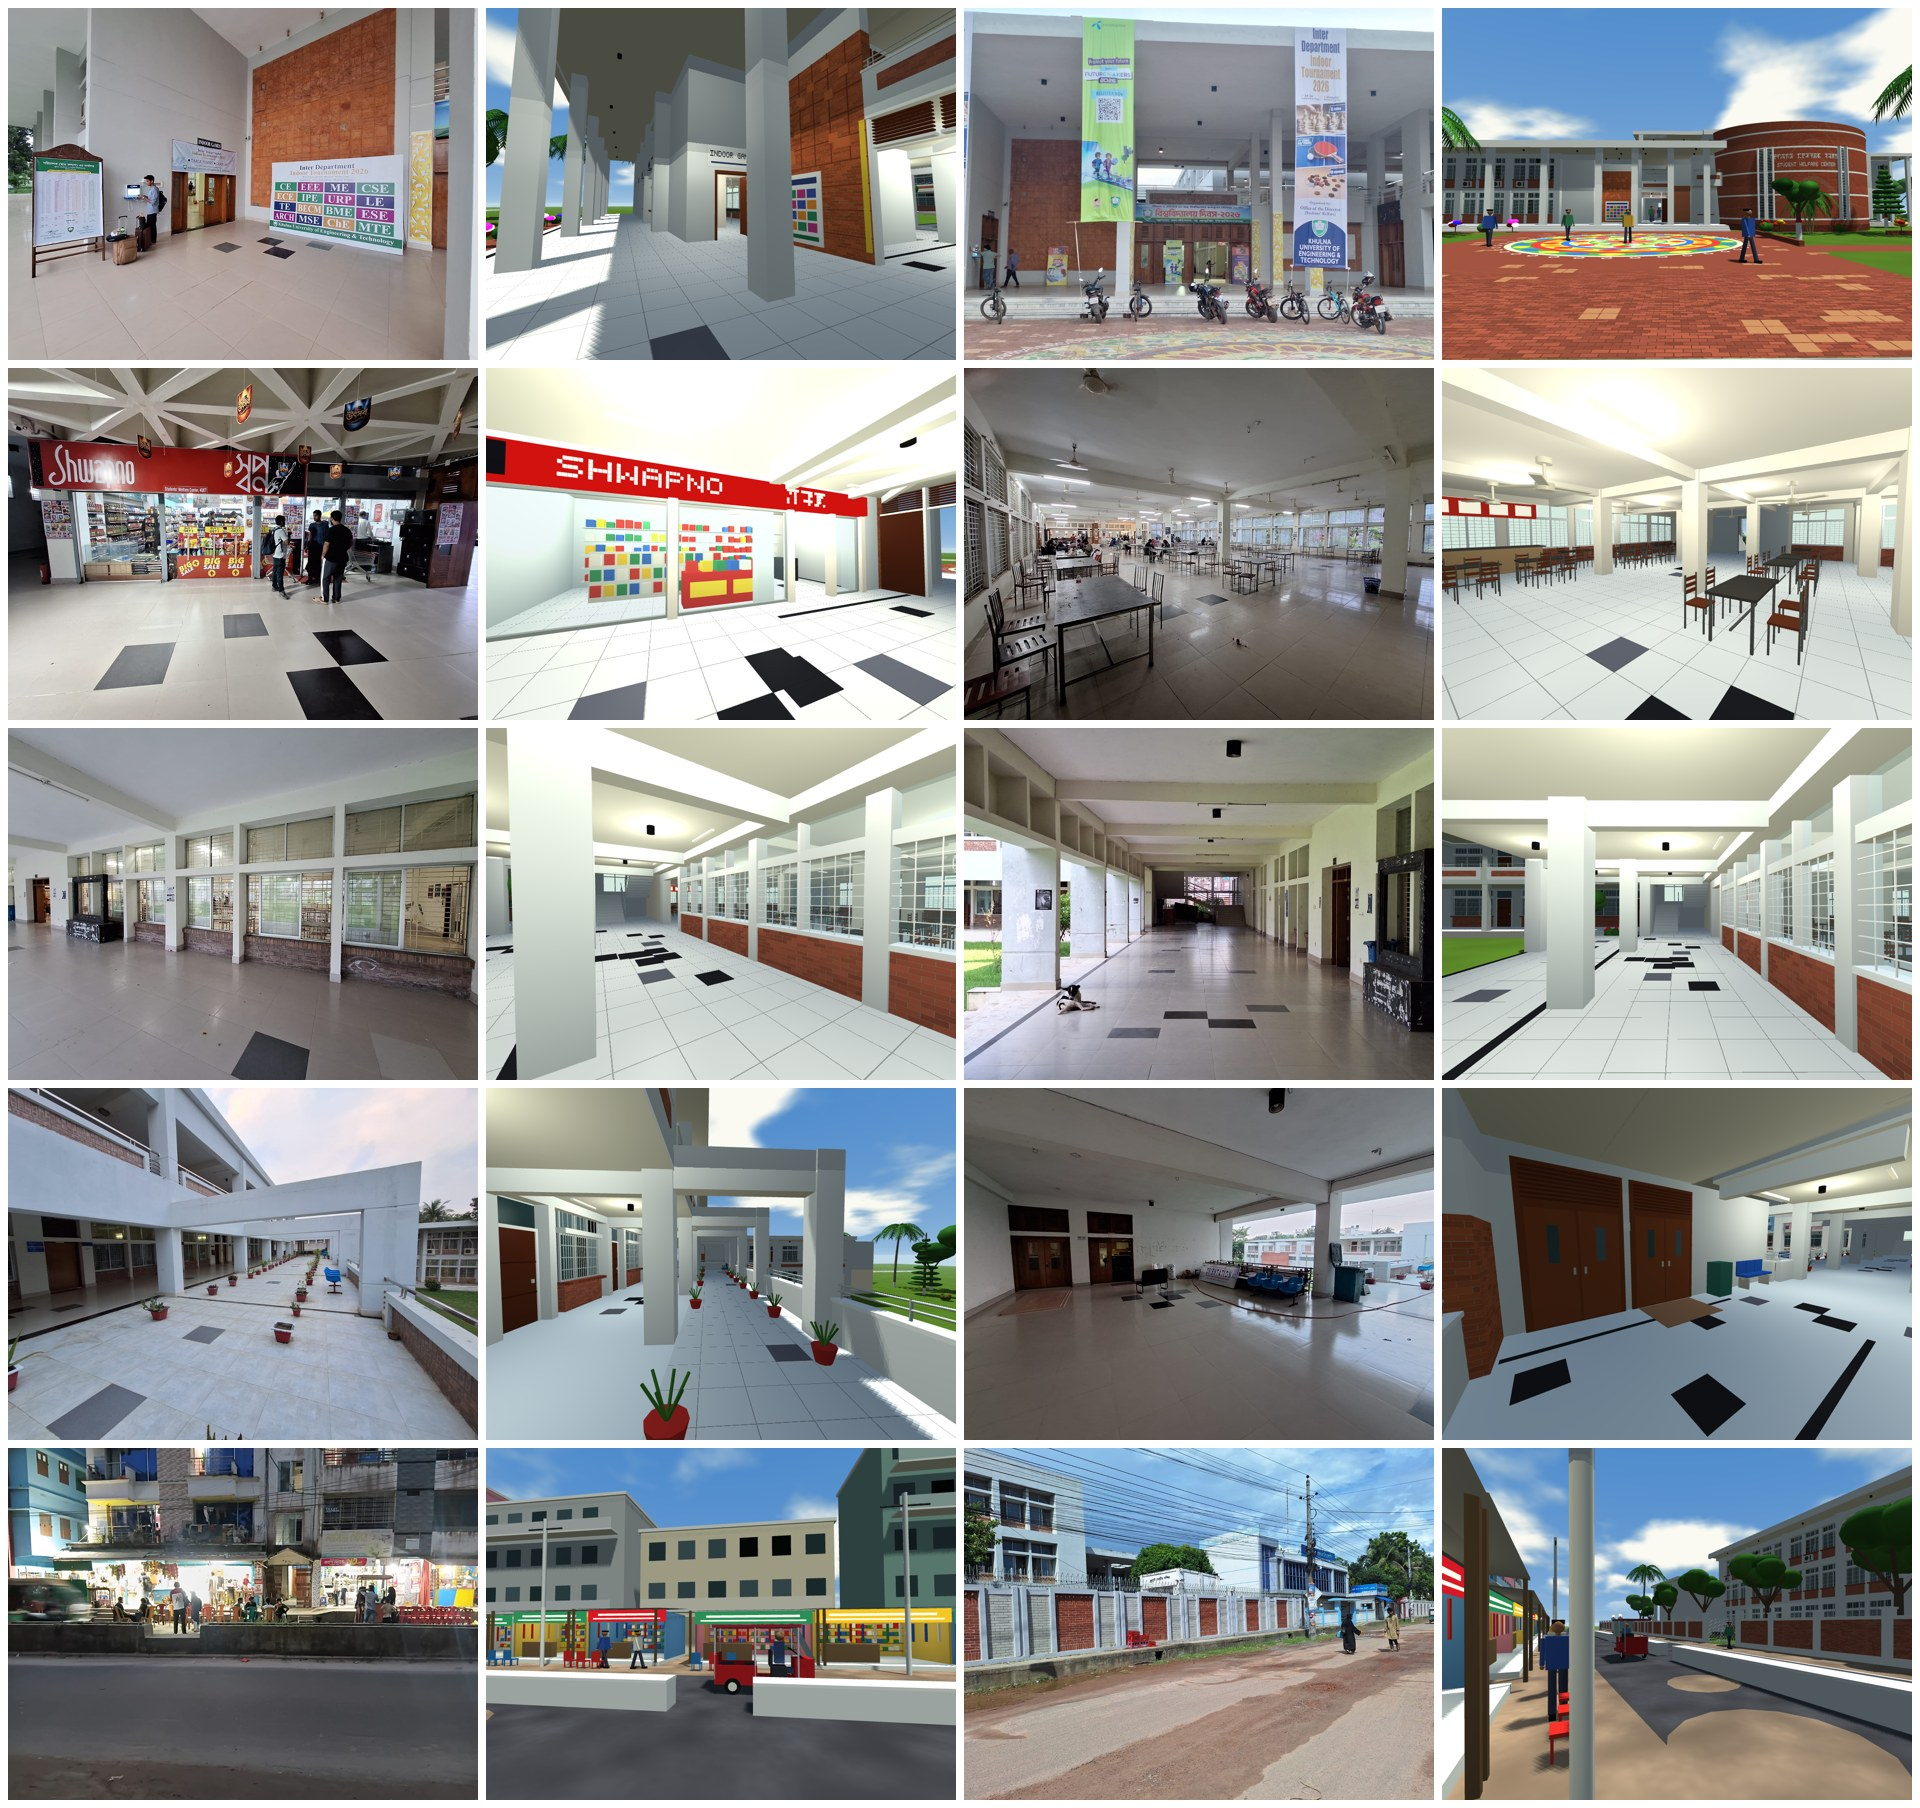
\includegraphics[width=0.90\textwidth]{photo-comparison.jpg}
\caption{Photographs (left of each pair) beside the model (right): lobby
and entrance; shop and cafeteria; corridor windows and corridor-end stair;
terrace and first-floor hall; stalls and boundary wall.}\label{fig:compare}
\end{figure}

\subsection{Scene statistics and interaction}
\begin{table}[H]
\centering\small
\begin{tabular}{@{}lr@{\hspace{2.2em}}lr@{}}
\toprule
Quantity & Value & Quantity & Value \\
\midrule
Reference photographs & 93 & Point lights & 113 \\
Triangles & about 367{,}000 & Ceiling fans & 21 \\
Source lines (C++/GLSL) & about 6{,}200 & Vehicles & 7 \\
Preset views & 37 & Pedestrians & 35 \\
Shadow map & $4096\times4096$ & Automatic tests & 3 \\
\bottomrule
\end{tabular}
\caption{Size of the finished project.}
\end{table}

The user can orbit, pan and zoom with the mouse; rotate, scale and
translate the whole model with the keyboard; jump to any of 37 views; walk
through the building with \code{WASD}; toggle shadows; pause the animation;
and ray trace the current view with a single key. Any view can also be
saved to an image file from the command line, with either renderer.

\subsection{Testing}
Three automatic tests are provided. The first checks the triangle counts,
bounds and normals of the basic shapes. The second checks collision in a
small test world: doorways pass, walls block, movement slides along walls,
stairs change the eye height, and low ceilings block. The third walks fixed
routes through the full model, including both stairs up and down, every
hall, the terrace and the link between the wings, and confirms that glass
walls and parapets stop the walker. All three pass. The visual match with
the photographs, and the appearance of the moving objects, were judged by
eye; no test compares pixels.

% ---------------------------------------------------------------- 10
\section{Limitations and Future Work}
\begin{itemize}
\item \textbf{Dimensions are estimated} from photographs; nothing was
measured on site. The second-floor interior and the rooms behind closed
doors were not photographed and are not modelled.
\item \textbf{The street is partly generated.} Its position relative to the
building is assumed, and the stalls and town buildings are produced by rule
with varied sizes and colours, not copied one by one.
\item \textbf{Real-time lighting is simplified.} Point lights cast no
shadows in the rasteriser, and only the 24 nearest are used. Window glazing
seen from inside is a bright panel, so sunlight does not enter through it.
\item \textbf{The ray tracer is not physically complete.} It has no soft
shadows, no refraction through thick glass, and no indirect light beyond
the ambient and fill terms.
\item \textbf{Motion is simple.} Vehicles and people follow fixed paths,
do not avoid each other, and are not part of collision. Wheels do not spin,
and a walking figure alternates between two poses.
\end{itemize}
Natural extensions are shadowed point lights, a skeletal walk cycle, path
tracing for indirect light, and a surveyed plan to replace the estimated
dimensions.

% ---------------------------------------------------------------- 11
\section{Conclusion}
The project meets all eleven requirements of the course with code written
from first principles: primitives, vector and matrix mathematics, composite
and hierarchical transformations, a look-at camera, perspective projection,
interactive control and per-fragment Phong lighting. On that foundation it
builds a recognisable model of a real campus building, inside and out, that
can be explored on foot, and adds shadow mapping, procedural materials,
transparency, animation and collision detection. Implementing a ray tracer
over the same scene made the difference between the two rendering
approaches concrete: the rasteriser is fast but approximates shadows and
reflections, while the ray tracer computes them directly at a much higher
cost.

% ---------------------------------------------------------------- references
\begin{thebibliography}{9}\small
\bibitem{phong} B.~T. Phong, ``Illumination for computer generated pictures,'' \emph{Communications of the ACM}, vol.~18, no.~6, pp.~311--317, 1975.
\bibitem{williams} L.~Williams, ``Casting curved shadows on curved surfaces,'' \emph{Computer Graphics (SIGGRAPH~'78)}, vol.~12, no.~3, pp.~270--274, 1978.
\bibitem{whitted} T.~Whitted, ``An improved illumination model for shaded display,'' \emph{Communications of the ACM}, vol.~23, no.~6, pp.~343--349, 1980.
\bibitem{mt} T.~M\"oller and B.~Trumbore, ``Fast, minimum storage ray-triangle intersection,'' \emph{Journal of Graphics Tools}, vol.~2, no.~1, pp.~21--28, 1997.
\bibitem{schlick} C.~Schlick, ``An inexpensive BRDF model for physically-based rendering,'' \emph{Computer Graphics Forum}, vol.~13, no.~3, pp.~233--246, 1994.
\bibitem{hearn} D.~Hearn, M.~P. Baker and W.~R. Carithers, \emph{Computer Graphics with OpenGL}, 4th~ed. Pearson, 2011.
\bibitem{glfw} GLFW: an open-source library for OpenGL window and input handling. \url{https://www.glfw.org}
\end{thebibliography}

\end{document}
